\documentclass[acmsmall,screen,review]{acmart}
\usepackage{booktabs,multirow,tikz,siunitx,xspace}
\usetikzlibrary{positioning,arrows.meta,fit,shapes.misc}
\sisetup{group-minimum-digits=4}
\newcommand{\op}[1]{\textsc{#1}}
\newcommand{\khop}{$k$-hop\xspace}
\AtBeginDocument{\providecommand\BibTeX{{Bib\TeX}}}
\setcopyright{none}
\acmJournal{TOIS}

\begin{document}
\title[When the Graph Breaks]{When the Graph Breaks: A Controlled Error-Injection Study of How Knowledge-Graph Construction Errors Propagate in GraphRAG}

\author{Author One}
\affiliation{\institution{Institution}\country{Country}}
\author{Author Two}
\affiliation{\institution{Institution}\country{Country}}

\begin{abstract}
Graph-based retrieval-augmented generation (GraphRAG) answers questions from knowledge graphs that large language models (LLMs) extract from text. These graphs contain errors: missed facts, fragmented or conflated entities and false triples. So far, the effect of such errors on answers has only been observed, never controlled.

We embed the gold evidence of 600 multi-hop questions from 2WikiMultihopQA in a realistic LLM-extracted graph and inject six typed construction errors, each at rates from 10\% to 50\%. We then trace every error through two retrievers, two context formats and five generators (123,487 answers).

Graph errors dominate. They explain 83--97\% of the variance in accuracy, compared with 8\% for the retriever and less than 1\% for the generator. Missing entities and edges are the most damaging: at a 30\% rate, accuracy falls from 0.89 to 0.26 and 0.40. These omissions act through retrieval and turn answers into abstentions. Corrupted relations and merged entities act partly through generation and are the only errors that make models repeat false facts. Attaching source sentences to triples recovers up to 17 accuracy points and cuts the odds of adopting false facts by about 60\%, whereas stronger generators do not help. Real LLM extractors miss 21--31\% of gold facts, which places them in the most damaging regime.

For multi-hop factoid question answering, the bottleneck of GraphRAG is graph construction, not the generator.
\end{abstract}

\begin{CCSXML}
<ccs2012><concept><concept_id>10002951.10003317</concept_id><concept_desc>Information systems~Information retrieval</concept_desc><concept_significance>500</concept_significance></concept>
<concept><concept_id>10010147.10010178.10010187</concept_id><concept_desc>Computing methodologies~Knowledge representation and reasoning</concept_desc><concept_significance>300</concept_significance></concept></ccs2012>
\end{CCSXML}
\ccsdesc[500]{Information systems~Information retrieval}
\ccsdesc[300]{Computing methodologies~Knowledge representation and reasoning}
\keywords{GraphRAG, knowledge graph construction, error propagation, retrieval-augmented generation, entity resolution, robustness, controlled experiment}

\maketitle

\section{Introduction}
Retrieval-augmented generation (RAG) grounds large language models (LLMs) in external evidence~\cite{lewis2020rag}. GraphRAG extends this idea by first turning a corpus into a knowledge graph and then retrieving entities, relations, paths or communities from it~\cite{edge2024local,peng2025survey,han2024graphrag}. The promise is better multi-hop reasoning and corpus-level sense-making~\cite{edge2024local,gutierrez2024hipporag,guo2025lightrag}. Controlled comparisons published since 2025, however, give a more cautious picture. GraphRAG and vector RAG behave in complementary ways and neither wins consistently~\cite{han2026ragvs,xiang2025when,zhou2025indepth}. Structure-augmented methods can fall below strong embedding retrieval on simple factual questions~\cite{gutierrez2025rag2memory}, and many reported gains shrink once the evaluation is debiased~\cite{zeng2025significant}.

One explanation for these mixed results recurs across the literature: the graph itself. Han et~al.\ report that only about two thirds of answer entities appear in LLM-constructed graphs for HotpotQA and Natural Questions~\cite{han2026ragvs}. Converting text to triples discards context~\cite{huang2025tcrqf}. Entity-resolution errors inflate and distort extracted graphs~\cite{cai2025extraction}. A few manipulated words at the extraction stage can poison downstream answers~\cite{wen2025fewwords,liang2025underfire}. Despite this, most evidence on construction errors is observational: the quality of the constructed graph is measured, or a mitigation is proposed and validated by end-task accuracy. Where errors have been manipulated directly, the manipulation is either adversarial, as in poisoning attacks~\cite{wen2025fewwords,liang2025underfire}, or limited to removing triples from curated KGs~\cite{zhou2025incomplete,wang2026missdiag}. No study has varied the error types characteristic of LLM extraction, such as split or conflated entities and plausible false triples, at controlled rates and traced them through the pipeline. As a result, three questions that determine engineering priorities remain open:
(i)~which construction errors matter, and how much; (ii)~whether their damage arises in retrieval or in generation; and (iii)~whether better retrievers, richer context or stronger generators can absorb them.

This paper closes that gap with a controlled error-injection study. We construct a \emph{gold-anchored graph} for 600 questions from 2WikiMultihopQA~\cite{ho2020twowiki}. The gold evidence triples of each question are embedded, exactly once and with sentence-level provenance, in a background graph that an LLM extracted from all 3,980 context paragraphs. This gives full control over every fact a question depends on, while keeping three properties of a real extracted graph: hub entities with very many connections, distractor facts about similar but irrelevant entities, and the extractor's own errors (Section~\ref{sec:anchor}). We then apply six seeded error operators that mirror the failure modes reported in the literature: entity deletion, edge deletion, entity split, entity merge, relation corruption and spurious edges. Each operator is applied at four rates between 10\% and 50\% of the graph's nodes or edges, and its effect is compared with the clean graph and traced through two retrievers, two context formats and five generators.

We fixed three research questions, their hypotheses and the analysis plan in a written protocol before running the main experiments; the protocol and its deviations log are released with the code. The study makes four contributions.

\begin{itemize}
\item \textbf{A controlled testbed.} We introduce a gold-anchored error-injection methodology for GraphRAG with typed operators, mediation-ready logging and a validated single-answer judge. Code and data are available at \url{https://github.com/ANONYMIZED/graphrag-error-injection}.
\item \textbf{Dose--response evidence.} We report curves for six construction error types. Omissions dominate: at a 30\% rate, entity deletion reduces accuracy from 0.89 to 0.26 and edge deletion to 0.40. Spurious edges are harmless under relation-aware retrieval.
\item \textbf{Stage attribution.} Graph errors explain 83--97\% of the variance in accuracy, against 8\% for the retriever and under 1\% for the generator. The loss from omission errors is mediated almost entirely by retrieval, whereas commission errors are the only ones that lead models to adopt false values.
\item \textbf{Calibration against real extractors.} The natural error profiles of three LLM extractors fall in the omission-dominated regime, and the injected curves give a conservative bound on accuracy over naturally extracted graphs.
\end{itemize}

Section~\ref{sec:related} reviews related work and Section~\ref{sec:design} states the research questions and hypotheses. Sections~\ref{sec:method} and~\ref{sec:setup} describe the method and the experimental setup. Section~\ref{sec:results} reports the results, Section~\ref{sec:discussion} discusses implications and Section~\ref{sec:threats} discusses threats to validity.

\section{Related Work}\label{sec:related}
\subsection{GraphRAG and KG-augmented generation}
GraphRAG covers two families~\cite{peng2025survey,han2024graphrag,pan2024unifying}. Text-derived graph indices build an entity graph from the corpus with an LLM. Examples are community summaries for query-focused summarization~\cite{edge2024local}, dual-level keyword retrieval~\cite{guo2025lightrag} and personalized-PageRank (PPR) retrieval inspired by hippocampal memory~\cite{gutierrez2024hipporag,gutierrez2025rag2memory}. KG-RAG methods instead reason over curated KGs, through LLM-guided exploration~\cite{sun2023tog}, relation-path planning~\cite{luo2023rog}, GNN or subgraph retrievers~\cite{he2024gretriever,mavromatis2025gnnrag} and lightweight subgraph scoring~\cite{li2024subgraphrag}. Modular decompositions such as LEGO-GraphRAG~\cite{cao2025lego} and the unified framework of Zhou et~al.~\cite{zhou2025indepth} split pipelines into graph building, indexing, operators and retrieval. However, they vary the methods operating on graphs, not the quality of the graph itself.

\subsection{Evaluations of GraphRAG}
Systematic comparisons find that GraphRAG helps on multi-hop and aggregation questions but often trails vanilla RAG on single-hop and detail-oriented ones~\cite{han2026ragvs,xiang2025when}. Agentic search narrows the gap to dense RAG~\cite{fan2026still}. Simpler or agentic pipelines can be competitive in production settings~\cite{chen2026needed}. Evaluation itself is fragile: LLM-as-judge comparisons show position, length and trial biases~\cite{zeng2025significant,zheng2023judge}, and KGQA benchmarks contain many incorrect labels~\cite{zhang2025pitfalls}. Our design responds to both problems. It uses single-answer judging against gold labels, which avoids pairwise position bias, and it validates the judge against a second model with adjudication.

\subsection{Construction errors and robustness}
Errors in LLM-based KG construction include missed facts, lost context~\cite{huang2025tcrqf}, entity fragmentation and conflation~\cite{cai2025extraction,christophides2021er} and noisy triples, which degrade downstream hallucination detection~\cite{kumar2026hallubench}. Graph-refinement research has long catalogued such errors for curated KGs~\cite{paulheim2017refinement}, and KG-embedding studies show sensitivity to sparsity and noise~\cite{pujara2017sparsity}. For KG-RAG, robustness to missing knowledge has been evaluated by random or typed removal of triples~\cite{zhou2025incomplete,wang2026missdiag}. GraphRAG-specific mitigations filter noisy retrievals and rebalance parametric knowledge~\cite{guo2025graphragfi}. Retrieval over-expansion is a further reported failure: graph retrieval raises recall but lowers relevance~\cite{wu2026memgraphrag}. In the security literature, adversarial attacks on the extraction step~\cite{liang2025underfire,wen2025fewwords} and data-extraction attacks~\cite{liu2025privacy} show that the graph is an attack surface in its own right. In plain RAG, noise robustness and the position of evidence in the context have been studied extensively~\cite{chen2024rgb,cuconasu2024power,liu2024lost,xie2023adaptive,zou2024poisonedrag}. Our study is the first, to our knowledge, to vary several typed \emph{construction} errors at controlled rates and to separate their retrieval-stage effects from their generation-stage effects.

\section{Research Questions and Hypotheses}\label{sec:design}
We fixed the research questions, hypotheses and analysis plan in a written protocol before running the main experiments. A pilot on 60 questions was used only to set the scale of the study. Deviations from the protocol are logged in the released materials and summarized in Section~\ref{sec:threats}. Each research question has one directional hypothesis, ordered by the expected importance of the answer for GraphRAG practice.

\begin{description}
\item[RQ1 (impact)] Which construction errors harm answer quality, and how much compared with the choice of retriever, context format and generator?\\
\textbf{H1.} Every error type reduces accuracy monotonically with its rate. Within realistic rates ($p\le0.3$), graph errors explain more variance in accuracy than any other factor.
\item[RQ2 (mechanism)] Through which pipeline stage does each error act, and how does it show in the answers?\\
\textbf{H2.} Omission errors (deletion, split) act mainly through retrieval and lead to abstentions. Commission errors (merge, corruption, spurious edges) act mainly through generation and lead to adoption of false values.
\item[RQ3 (mitigation)] Can richer context or stronger generators absorb the damage?\\
\textbf{H3.} Attaching source sentences reduces false-value adoption under commission errors but not the loss under omission errors. Stronger generators reduce generation-stage loss but not retrieval-stage loss.
\end{description}

In addition, an exploratory analysis (Section~\ref{sec:natural}) tests whether curves obtained by uniform injection predict accuracy over graphs built entirely by an LLM extractor.

\section{Method}\label{sec:method}
\begin{figure}[t]
\centering
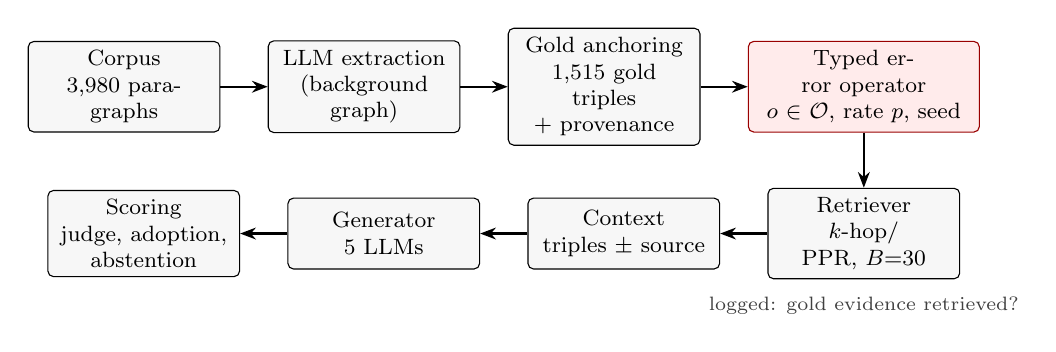
\begin{tikzpicture}[node distance=4mm and 6mm, every node/.style={font=\footnotesize},
 box/.style={draw, rounded corners=2pt, align=center, minimum height=9mm, text width=22mm, fill=gray!6},
 inj/.style={draw=red!60!black, fill=red!8, rounded corners=2pt, align=center, text width=27mm, minimum height=9mm},
 arr/.style={-{Stealth[length=2mm]}, thick}]
\node[box] (corp) {Corpus\\3,980 paragraphs};
\node[box, right=of corp] (bg) {LLM extraction\\(background graph)};
\node[box, right=of bg] (anch) {Gold anchoring\\1,515 gold triples\\+ provenance};
\node[inj, right=of anch] (op) {Typed error operator\\$o \in \mathcal{O}$, rate $p$, seed};
\node[box, below=7mm of op] (ret) {Retriever\\\khop / PPR, $B{=}30$};
\node[box, left=of ret] (ctx) {Context\\triples $\pm$ source};
\node[box, left=of ctx] (gen) {Generator\\5 LLMs};
\node[box, left=of gen] (eval) {Scoring\\judge, adoption,\\abstention};
\draw[arr] (corp)--(bg); \draw[arr] (bg)--(anch); \draw[arr] (anch)--(op); \draw[arr] (op)--(ret);
\draw[arr] (ret)--(ctx); \draw[arr] (ctx)--(gen); \draw[arr] (gen)--(eval);
\node[below=1mm of ret, font=\scriptsize, text=gray!50!black] {logged: gold evidence retrieved?};
\end{tikzpicture}
\caption{Study design. Gold evidence triples are embedded exactly once in an LLM-extracted background graph. One typed error operator is then applied at a controlled rate, and its effect is traced through retrieval, context assembly, generation and scoring. Logging whether the gold evidence was retrieved lets us split the accuracy loss into a retrieval component and a generation component.}
\label{fig:design}
\end{figure}

\subsection{Gold-anchored graph}\label{sec:anchor}
\paragraph{Data.} 2WikiMultihopQA~\cite{ho2020twowiki} provides, for each question, gold evidence triples (e.g., \emph{(Polish-Russian War; director; Xawery \.Zu\l{}awski)}), supporting sentences and ten context paragraphs, eight of which are distractors. Unlike HotpotQA~\cite{yang2018hotpotqa} or MuSiQue~\cite{trivedi2022musique}, it supplies explicit evidence triples. These triples act as a gold sub-graph whose integrity we can control. We drew 600 development questions, stratified evenly across the four question types: compositional, inference, comparison and bridge-comparison. The corpus is the union of their context paragraphs (3,980 unique paragraphs, 14,623 sentences), so distractors from all questions compete in retrieval.

\paragraph{Background graph.} An LLM extractor (gpt-oss-120b) produced (sentence, subject, relation, object) quadruples from every paragraph. The prompt was schema-guided, with relation labels taken from the dataset vocabulary and other labels allowed, and the extraction yielded 33,468 triples. Entity mentions were normalized and resolved to gold entity names and paragraph titles, by exact normalized match or by fuzzy match (ratio $\ge 94$).

\paragraph{Anchoring.} We removed the 1,393 background triples that duplicated a gold fact, i.e.\ triples with the same head--tail pair, or the same head and relation, as a gold triple. We then inserted the 1,515 unique gold triples, each with the supporting sentence that states it as provenance. In the resulting graph $G^\star$ (33,217 edges, 26,474 nodes), every fact a question depends on exists exactly once. Each injected error therefore has an unambiguous counterfactual, while the background graph supplies three properties of real extracted graphs that make retrieval hard. We use the terms as follows. \emph{Hubs} are nodes of very high degree, in the sense of network science, that connect otherwise unrelated questions; the largest is \emph{United States} with 397 incident edges, followed by \emph{American} (272) and \emph{film director} (247). \emph{Distractors} are facts about entities that are similar to, but irrelevant for, a question; they come mainly from the eight distractor paragraphs that 2WikiMultihopQA attaches to each question, a term the dataset inherits from the distractor setting of HotpotQA~\cite{yang2018hotpotqa}. \emph{Noise} denotes the extractor's own errors: imprecise or unsupported triples, about 3\% of the background triples (Table~\ref{tab:natural}), and inconsistent surface forms of entities.

\subsection{Typed error operators}
Each operator $o$ is applied to $G^\star$ at rate $p \in \{0.1, 0.2, 0.3, 0.5\}$ with a fixed seed, sampling uniformly from all nodes or edges. Operators are applied one at a time; their interactions are left to future work. The six operators are:
\begin{itemize}
\item \op{Ent\_Del} removes $p|V|$ nodes together with their incident edges. It models missed entities.
\item \op{Edge\_Del} removes $p|E|$ edges. It models missed relations, the dominant natural error (Section~\ref{sec:natural}).
\item \op{Split} gives $p|V|$ nodes a surface-variant alias (an initialism, a reordered name or a qualifier). Each incident edge moves to the alias with probability 0.5. It models entity fragmentation.
\item \op{Merge} fuses $p|V|$ nodes with their most name-similar neighbour in a blocking key; the surviving label is chosen at random. It models over-eager entity resolution.
\item \op{Rel\_Corrupt} replaces the object of $p|E|$ edges with the object of a random edge that has the same relation, producing a plausible false fact. The original provenance sentence is kept, as a source pointer would be.
\item \op{Spurious} adds $p|E|$ edges with a random subject and a relation--object pair sampled from existing edges, together with a random sentence of the subject. It models hallucinated triples.
\end{itemize}
We group \op{Ent\_Del}, \op{Edge\_Del} and \op{Split} as \emph{omission} errors, which hide true facts, and \op{Merge}, \op{Rel\_Corrupt} and \op{Spurious} as \emph{commission} errors, which assert false structure.

\subsection{Retrieval, context and generation}
\paragraph{Entity linking.} Both retrievers link question $n$-grams (up to 12 tokens) to node names by exact normalized match, with the longest match taking priority. Linking is deliberately not fuzzy, so that split and merge errors act on linking in the way they would in a production pipeline that indexes canonical labels.

\paragraph{Retrievers.} \khop expands up to two hops from the seed nodes. It ranks edges by hop distance and by a lexical match between relation labels and question cues (e.g., ``born'' $\rightarrow$ \emph{date/place of birth}). PPR follows HippoRAG~\cite{gutierrez2024hipporag}: it runs personalized PageRank (damping 0.5) from the seed nodes and scores each two-hop candidate edge by the PPR mass of its endpoints times the same relation match. Both retrievers return the top $B=30$ triples.

\paragraph{Context.} Retrieved triples are serialized as \emph{(subject; relation; object)}. In the \emph{provenance} condition each triple is followed by its source sentence.

\paragraph{Generation.} The generator is instructed to answer from the facts only and to reply ``insufficient information'' when the facts do not suffice. It returns a short final answer at temperature 0.

\subsection{Outcomes}
\paragraph{Primary outcome.} Accuracy is judged against the gold answer. Abstentions count as incorrect, and exact matches are accepted without calling the judge. All remaining answers (3,953 unique question--answer pairs) are labelled by a single-answer judge, deepseek-v4.1-flash, a model family not used for generation. On a random sample of 300 non-trivial items, the judge agreed with an independent second judge (Claude Sonnet~4.6) on 97\% of cases (Cohen's $\kappa=0.94$). After adjudicating the disagreements with a third model, the primary judge was correct on 98\% of the sample.

\paragraph{Secondary outcomes.}
\begin{itemize}
\item \emph{Abstention}: the generator replies ``insufficient information''.
\item \emph{False-value adoption}: an incorrect answer that matches an injected false value present in the context.
\item \emph{Gold evidence retrieved}: all of the question's gold edges are in the context, possibly in corrupted form.
\end{itemize}

\subsection{Analysis}
\paragraph{Dose--response (H1).} Rate slopes are estimated with population-averaged logistic GEE models (exchangeable working correlation within questions):
\begin{equation}
\operatorname{logit}\Pr(\text{correct}) = \beta_0 + \sum_{o\in\mathcal{O}} \beta_o\, p\,\mathbb{1}[\text{op}=o] + \gamma_{\text{ret}} + \gamma_{\text{prov}} + \gamma_{\text{type}},
\end{equation}
with Holm correction across the six slopes. Slopes of gold-evidence retrieval come from the deterministic retrieval grid (rates 0--0.5 in steps of 0.05--0.1, three seeds), with question-clustered standard errors.

\paragraph{Variance decomposition (H1).} Condition-level accuracies are decomposed with Shapley values of $R^2$ over the factors graph condition (operator $\times$ rate), retriever, provenance and generator.

\paragraph{Mediation (H2, H3).} For a condition $c$ and the clean graph $0$, let $s$ be the probability that the gold evidence is retrieved and $a_s$, $a_{\bar s}$ the accuracy with and without it. We decompose the accuracy drop into a retrieval term $(s_0 - s_c)(a_{s,0} - a_{\bar s,0})$ and a generation term (the remainder). Confidence intervals come from a question-level bootstrap with 1,000 resamples.

\paragraph{Outcomes and moderation (H2, H3).} Differences in the outcome distribution (correct, abstained, adopted false value, other wrong) are tested with $\chi^2$ tests. The moderating effects of provenance and generator are tested with GEE interaction terms.

\section{Experimental Setup}\label{sec:setup}
\paragraph{Generators.} Claude Haiku~4.5 is the primary generator and runs the full grid: 25 graph conditions (clean graph plus 6 operators $\times$ 4 rates) $\times$ 2 retrievers $\times$ 2 context formats $\times$ 600 questions, i.e.\ 60,000 answers. Three open-weight models run the \khop grid (clean graph and rates 0.1 and 0.3, both context formats): gpt-oss-120b, gpt-oss-20b and Gemma~4~31B. Claude Sonnet~4.6 runs the clean graph and rate 0.3.

\paragraph{Reference systems.} All generators also answer closed-book (no retrieval) and with dense passage RAG, which retrieves the top five paragraphs by TF-IDF from the full corpus.

\paragraph{Natural graphs.} For the exploratory analysis, we built graphs entirely from extractor output (gpt-oss-120b and Claude Haiku~4.5), without gold anchoring, and answered all questions over them with Haiku and \khop retrieval.

\paragraph{Scale and cost.} In total the study comprises 123,487 generated answers. All model calls are cached and reproducible from the released prompts.

\section{Results}\label{sec:results}
\paragraph{Baselines.} On the clean gold-anchored graph, \khop retrieves the complete gold evidence for 89.2\% of the questions and PPR for 75.8\%. The remaining failures stem mostly from naming inconsistencies in the dataset's own evidence. With Haiku, clean-graph accuracy is 0.892 (95\% CI 0.867--0.915) with \khop and 0.760 with PPR. This is far above dense passage RAG (0.327) and closed-book answering (0.208). Closed-book accuracy varies widely across generators, from 0.21 for Haiku and gpt-oss-20b to 0.58 for Sonnet~4.6. Under graph-grounded instructions, however, all five generators reach the same clean-graph accuracy (0.88--0.90; Table~\ref{tab:main}, Figure~\ref{fig:attr}b).

\subsection{RQ1: Which errors matter}
\paragraph{Dose--response.}
\begin{figure}[t]
\centering
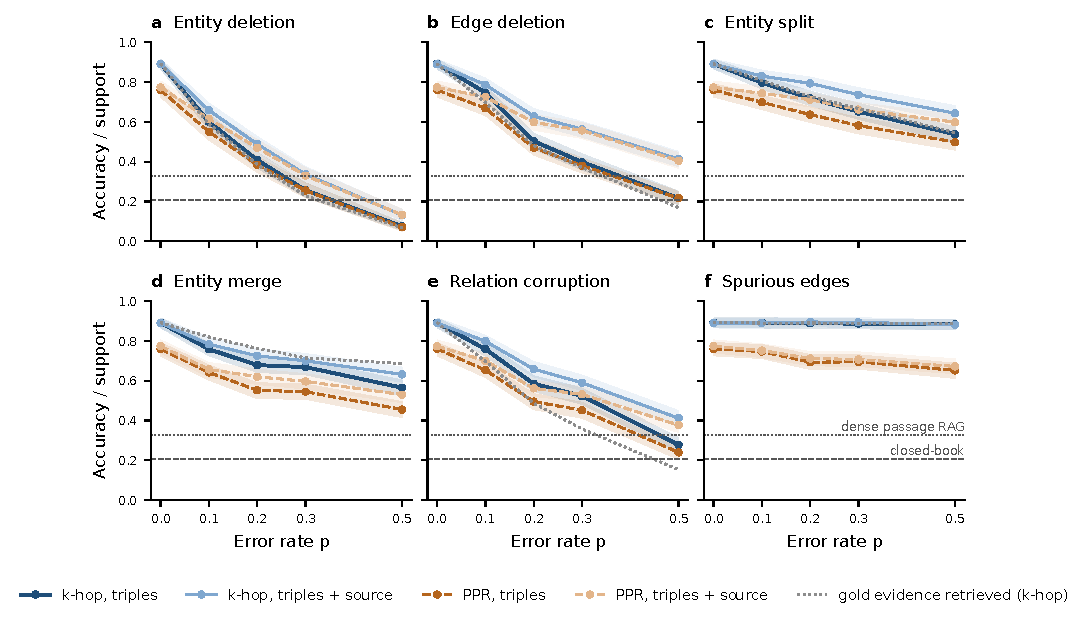
\includegraphics[width=\linewidth]{figures/fig2_dose_response.pdf}
\caption{Accuracy of Claude Haiku~4.5 as a function of the error rate $p$, for each operator, retriever and context format (600 questions per point; shaded bands are question-cluster bootstrap 95\% CIs). The dotted grey line shows the share of questions whose complete gold evidence is retrieved by \khop (mean over three seeds). Horizontal reference lines show dense passage RAG and closed-book accuracy for the same generator.}
\label{fig:dose}
\end{figure}

\begin{table}[t]
\caption{Accuracy (Claude Haiku~4.5) at $p=0.3$ and per-operator rate effects. The odds ratio (OR) per $+0.1$ in error rate comes from the GEE model (Holm-adjusted $p$). The retrieval slope is the change in the share of questions with complete gold evidence retrieved per unit of rate (\khop, three seeds).}
\label{tab:main}
\small
\begin{tabular}{lccccccc}
\toprule
& \multicolumn{2}{c}{\khop} & \multicolumn{2}{c}{PPR} & \multicolumn{2}{c}{Rate effect} & Retrieval \\
\cmidrule(lr){2-3}\cmidrule(lr){4-5}\cmidrule(lr){6-7}
Operator & triples & + source & triples & + source & OR/0.1 & $p_{\text{Holm}}$ & slope \\
\midrule
Clean graph & 0.892 & 0.890 & 0.760 & 0.775 & -- & -- & -- \\
\op{Ent\_Del} & 0.257 & 0.337 & 0.255 & 0.329 & 0.35 & $<10^{-99}$ & $-1.52$ \\
\op{Edge\_Del} & 0.398 & 0.563 & 0.380 & 0.557 & 0.58 & $<10^{-66}$ & $-1.44$ \\
\op{Split} & 0.652 & 0.737 & 0.582 & 0.663 & 0.79 & $<10^{-29}$ & $-0.66$ \\
\op{Merge} & 0.668 & 0.700 & 0.545 & 0.598 & 0.72 & $<10^{-30}$ & $-0.38$ \\
\op{Rel\_Corrupt} & 0.523 & 0.590 & 0.452 & 0.533 & 0.65 & $<10^{-58}$ & $-1.45$ \\
\op{Spurious} & 0.887 & 0.893 & 0.695 & 0.707 & 1.01 & 0.43 & $-0.01$ \\
\bottomrule
\end{tabular}
\end{table}

Five of the six operators reduce accuracy monotonically (Figure~\ref{fig:dose}, Table~\ref{tab:main}). The steepest decline comes from entity deletion: each additional 10\% of deleted entities multiplies the odds of a correct answer by 0.35. At $p=0.3$, accuracy falls from 0.892 to 0.257 (95\% CI 0.222--0.293) and abstention rises to 72\%. Edge deletion follows (OR 0.58; 0.398 at $p=0.3$), then relation corruption (0.65; 0.523), merge (0.72; 0.668) and split (0.79; 0.652).

The ranking follows how many gold elements each operator can break. A question depends on two to four gold edges and three to six gold nodes. Deleting a node removes all of its edges, so each gold node is a single point of failure. A split, by contrast, disconnects only the half of a node's edges that move to the alias. Spurious edges have no detectable effect with \khop (OR 1.01, $p=0.43$). Because \khop ranks edges by relation match, a random extra triple rarely displaces a gold triple. With PPR, which rewards graph centrality, the same operator lowers accuracy by up to 11 points at $p=0.5$, showing that the harm of hallucinated triples depends on the retriever.

The protocol also predicted that omission operators would lower gold-evidence retrieval more steeply than commission operators. This holds only in part. The two deletion operators lower gold-evidence retrieval most steeply (slopes $-1.52$ and $-1.44$), and split lowers it more than merge or spurious edges. However, relation corruption lowers retrieval as steeply as edge deletion ($-1.45$). The reason is that a corrupted first-hop edge redirects a two-hop traversal to the wrong intermediate entity, so the second gold edge is never reached. Corruption thus acts as an omission error on the downstream hop.

\paragraph{Question type.} The damage depends on how many facts a question needs (Table~\ref{tab:qtype}). Bridge-comparison questions need four gold facts, and at $p=0.3$ their accuracy under entity deletion falls from 0.92 to 0.13. Comparison questions need two independent one-hop facts and keep 0.78--0.82 accuracy under merge and corruption, partly because their binary answers can be guessed.

\begin{table}[t]
\caption{Accuracy by question type on the clean graph and at $p=0.3$ (Claude Haiku~4.5, \khop, triples only; 150 questions per type).}\label{tab:qtype}
\small
\begin{tabular}{lccccccc}
\toprule
Type (gold facts) & Clean & \op{Ent\_Del} & \op{Edge\_Del} & \op{Split} & \op{Merge} & \op{Rel\_Corrupt} & \op{Spurious}\\
\midrule
Comparison (2) & 1.000 & 0.273 & 0.533 & 0.800 & 0.780 & 0.820 & 0.993 \\
Compositional (2) & 0.853 & 0.300 & 0.413 & 0.647 & 0.620 & 0.427 & 0.847 \\
Inference (2) & 0.793 & 0.327 & 0.413 & 0.627 & 0.673 & 0.400 & 0.787 \\
Bridge-comparison (4) & 0.920 & 0.127 & 0.233 & 0.533 & 0.600 & 0.447 & 0.920 \\
\bottomrule
\end{tabular}
\end{table}

\paragraph{Comparison with other design choices.}\begin{figure}[t]
\centering
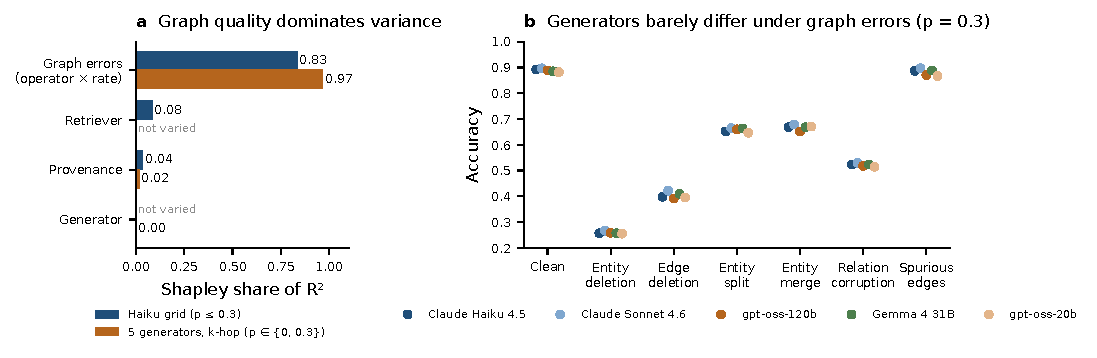
\includegraphics[width=\linewidth]{figures/fig4_attribution.pdf}
\caption{(a) Shapley decomposition of the explained variance in condition-level accuracy, for the Haiku grid ($p\le 0.3$; factors: graph condition, retriever, provenance) and for the five-generator grid (\khop; $p\in\{0,0.3\}$; factors: graph condition, generator, provenance). (b) Accuracy of the five generators on the clean graph and at $p=0.3$ for each operator (\khop, triples only, 600 questions each).}
\label{fig:attr}
\end{figure}

The second part of H1 is strongly supported (Figure~\ref{fig:attr}a). Across the Haiku grid with $p \le 0.3$, the graph condition accounts for a Shapley share of 0.83 of condition-level $R^2$ (total $R^2=0.95$). The retriever accounts for 0.08 and provenance for 0.04. In the five-generator grid the graph condition accounts for 0.97, provenance for 0.02 and the generator for 0.003. Because the graph factor spans more levels than the other factors, we also compare effects at matched magnitudes. At the mildest error rate tested ($p=0.1$), the mean accuracy loss across the six operators (0.133) already equals the clean-graph gap between \khop and PPR (0.132) and is about nine times the largest clean-graph difference between generators (0.015). At $p=0.3$ the mean loss is 0.328. At the level of individual questions, the graph condition also explains more deviance (McFadden $R^2=0.067$) than question type (0.049), retriever (0.007) or provenance (0.003).

The generators are close to interchangeable (Figure~\ref{fig:attr}b). Averaged over the three omission operators at $p=0.3$, accuracy ranges from 0.47 (gpt-oss-120b) to 0.51 (Sonnet~4.6); over the commission operators it ranges from 0.69 to 0.72. Sonnet's much stronger parametric knowledge (closed-book accuracy 0.58 versus 0.21 for Haiku) does not translate into robustness against graph errors under grounded instructions.

\subsection{RQ2: Where the damage arises}
\begin{figure}[t]
\centering
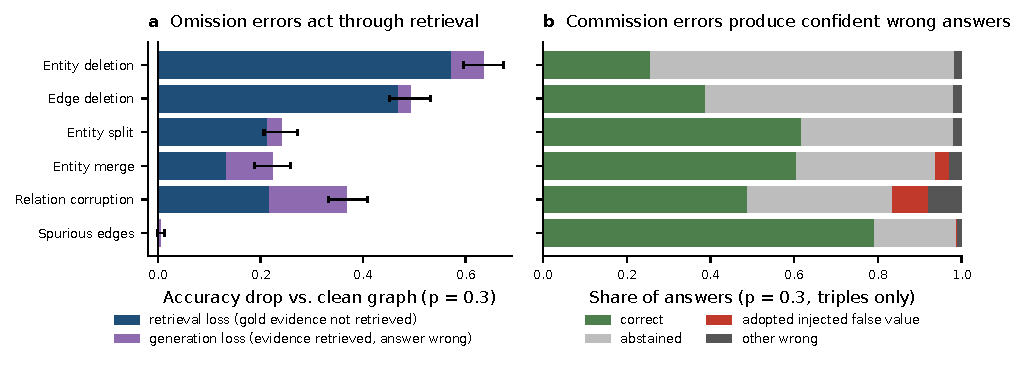
\includegraphics[width=\linewidth]{figures/fig3_mechanism.pdf}
\caption{(a) Decomposition of the accuracy drop at $p=0.3$ (Haiku, \khop, triples only) into a retrieval component (gold evidence no longer retrieved) and a generation component (evidence retrieved, possibly corrupted, but answer wrong). Error bars are bootstrap 95\% CIs of the total drop. (b) Distribution of outcomes for the same conditions.}
\label{fig:mech}
\end{figure}

The mediation decomposition separates two mechanisms (Figure~\ref{fig:mech}a). For the omission operators, almost all of the loss arises in retrieval. The retrieval share is 0.95 (95\% CI 0.84--1.04) for edge deletion, 0.90 (0.81--0.98) for entity deletion and 0.89 (0.78--0.99) for split, which supports H2 for omission errors. Once the gold evidence is missing, generators rarely recover, and they abstain rather than guess.

For relation corruption and merge, the retrieval shares are 0.59 (0.51--0.67) and 0.60 (0.48--0.74). The generation share is therefore about 0.40, below 50\%, so the generation part of H2 is not supported for these operators. Both commission errors also act through retrieval: corruption redirects traversals, and merges relabel nodes so that question entities no longer link. Even so, they are the only errors with a substantial generation-stage component. The shares are almost identical across the five generators (0.56--0.61 for merge and 0.58--0.60 for corruption) and similar for PPR. The mechanism is thus a property of the error, not of the model.

\subsection{RQ3: Mitigation}
\paragraph{Confident errors (H2, continued).} The outcome distribution differs sharply by error class ($\chi^2=1974$, df$=3$, $p<10^{-15}$; Figure~\ref{fig:mech}b). Pooled over both retrievers, among incorrect answers under omission errors, 97.2\% are abstentions, 2.8\% are other wrong answers and none adopts a false value. Under commission errors, 78.5\% are abstentions, 10.6\% adopt an injected false value and 10.9\% are other wrong answers. Under relation corruption at $p=0.3$, 8.8\% of all answers repeat the injected false object. Omission errors make a GraphRAG system less helpful; commission errors make it wrong with confidence. The outcome part of H2 is supported.

\paragraph{Provenance (H3).} Attaching source sentences reduces false-value adoption (OR 0.41, $p<10^{-27}$). For Haiku under corruption at $p=0.3$, adoption falls from 8.8\% to 3.5\%, because the kept sentence contradicts the corrupted triple. Contrary to the first part of H3, provenance helps most under \emph{omission}: under edge deletion at $p=0.3$, it raises accuracy by 16.5 points (0.398 to 0.563), and it recovers 8.5 points under split.

The mechanism is redundancy. A sentence attached to a surviving triple often also states the deleted fact; for example, a film's release-year sentence frequently names its director. The mediation analysis shows this as a negative generation component under provenance: the generator recovers facts that retrieval lost. The rate $\times$ provenance interaction is positive ($\beta=0.85$, $p<10^{-11}$). The three-way interaction with the commission indicator is negative ($\beta=-0.43$, $p=0.002$), so the benefit of provenance is smaller against commission errors. Its size also depends on the generator. Under corruption at $p=0.3$, provenance adds 6--7 points for the Claude models but only 1--3 points for gpt-oss-120b, Gemma~4 and gpt-oss-20b, which give the contradicting sentence less weight.

\paragraph{Generator strength (H3).} The second part of H3 is not supported. The generator $\times$ error-class interactions are not significant (all $p>0.07$), the mediation shares do not differ between generators, and generator choice explains less than 1\% of the variance. Within the tested range of capabilities, the stronger generator neither reduces generation-stage loss nor narrows the gap.

\subsection{Exploratory analysis: natural extraction errors}\label{sec:natural}
\begin{table}[t]
\caption{Natural error profiles of three LLM extractors on the supporting paragraphs (1,464 paragraphs). Coverage is the share of gold facts recovered as a triple linking the same head and tail. Tail conflict is the share of gold (head, relation) pairs extracted with a different object. The split rate is the share of gold entities with at least one surface variant among the extracted nodes. The unsupported share comes from a verifier check of 200 sampled triples per extractor.}
\label{tab:natural}
\small
\begin{tabular}{lcccccc}
\toprule
Extractor & Triples & Coverage (strict) & Coverage (any rel.) & Tail conflict & Split rate & Unsupported \\
\midrule
gpt-oss-120b & 16,274 & 0.589 & 0.690 & 0.050 & 0.136 & 0.030 \\
Claude Haiku 4.5 & 17,369 & 0.679 & 0.787 & 0.031 & 0.119 & 0.055 \\
Gemma 4 31B & 17,282 & 0.635 & 0.751 & 0.022 & 0.131 & 0.060 \\
\bottomrule
\end{tabular}
\end{table}

Real extractors operate in the omission-dominated regime (Table~\ref{tab:natural}). Even under a lenient criterion that accepts any relation label, 21--31\% of gold facts are never extracted as a triple linking the right entities. In contrast, only 2--5\% of extracted (head, relation) pairs carry a wrong object and 3--6\% of triples are unsupported by their paragraph. About 12--14\% of gold entities appear under more than one surface form. Mapped onto Figure~\ref{fig:dose}, the omission share alone corresponds to edge deletion at $p\approx0.2$--$0.3$, which is the steepest part of the curve.

\begin{figure}[t]
\centering
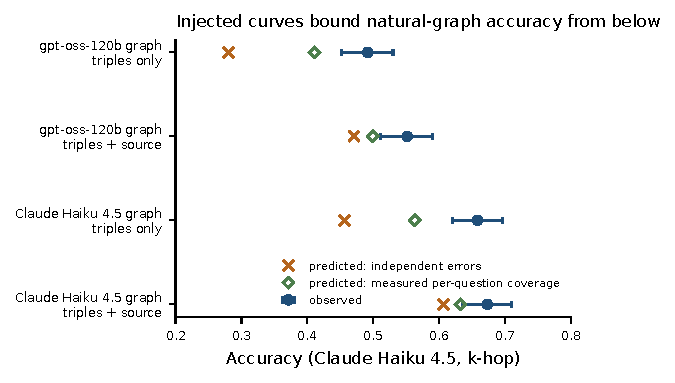
\includegraphics[width=0.62\linewidth]{figures/fig5_natural.pdf}
\caption{Observed accuracy (Haiku, \khop) over graphs built entirely by two extractors, with bootstrap 95\% CIs, compared with two predictions: an additive logit model fitted on the injected conditions and evaluated at the measured error profile (independent errors), and a mediation model using the measured per-question coverage of gold facts.}
\label{fig:natural}
\end{figure}

The exploratory prediction does not hold in its strict form (Figure~\ref{fig:natural}). Over graphs built only by an extractor, Haiku reaches 0.492 accuracy on the gpt-oss-120b graph and 0.658 on the Haiku graph with triples only, and 0.552 and 0.673 with provenance. These values sit far below the clean gold-anchored graph (0.892), but above the additive model's predictions of 0.280 and 0.456 with triples only.

Two properties of natural errors explain the gap, and a coverage-based prediction narrows it. First, natural omissions cluster within questions: the share of questions with all gold facts covered (0.40 and 0.58) exceeds what independent errors at the same per-fact coverage would give (0.36 and 0.49). Second, partially covered questions can sometimes still be answered. A mediation model that uses the measured per-question coverage predicts 0.411 and 0.563, within 0.04--0.10 of the observed values. With only two extractors and one generator, this comparison is indicative. The uniform-injection curves should be read as a conservative lower bound on the accuracy of real pipelines, not as a calibrated predictor.

\paragraph{Sensitivity analysis.} Restricted to the 535 questions with complete gold evidence on the clean graph, the clean accuracy is 0.987. The ranking of operators and every qualitative conclusion are unchanged; for example, accuracy at $p=0.3$ is 0.280 under entity deletion, 0.441 under edge deletion and 0.981 under spurious edges.

\begin{table}[t]
\caption{Summary of the hypothesis tests.}\label{tab:hyp}
\small
\begin{tabular}{p{0.9cm}p{5.6cm}p{6.3cm}}
\toprule
& Prediction & Outcome \\
\midrule
H1 & All error types reduce accuracy monotonically; graph errors explain the most variance & \textbf{Largely supported.} Five of six types reduce accuracy (spurious edges: no effect under \khop); Shapley share 0.83--0.97 vs.\ $\le$0.08 for every other factor \\
H2 & Omissions act through retrieval and cause abstention; commission errors act through generation and cause false-value adoption & \textbf{Partially supported.} Omissions: 89--95\% retrieval-mediated, 97\% of wrong answers are abstentions. Commission: only $\approx$40\% generation-mediated, but the only source of adoption (10.6\% of wrong answers) \\
H3 & Provenance reduces adoption but not omission loss; stronger generators reduce generation loss & \textbf{Mixed.} Provenance reduces adoption (OR 0.41) and, unexpectedly, helps most under omission (+16.5 pts); generators: no effect (share $<$1\%) \\
Expl. & Injected curves predict accuracy on natural graphs & \textbf{Not in strict form.} Curves are a conservative lower bound; a coverage-based model comes within 0.04--0.10 \\
\bottomrule
\end{tabular}
\end{table}

\section{Discussion}\label{sec:discussion}
\paragraph{The bottleneck is the graph.} Within the tested space, which is multi-hop factoid QA over Wikipedia-style text, the quality of the graph matters roughly ten times more than the choice of retriever and about a hundred times more than the choice among five generators that span model families and sizes. This puts the observational finding that GraphRAG ``underperforms on many tasks''~\cite{han2026ragvs,xiang2025when} on causal footing: a large part of the gap can come from construction, which current method papers rarely ablate. The practical implication is to measure graph coverage of the evidence needed for target questions before tuning retrievers or upgrading generators. Evaluation papers should likewise report graph-construction quality next to end-task accuracy, along the lines of the stage-wise metrics proposed by GraphRAG-Bench~\cite{xiang2025when}.

\paragraph{Omissions dominate in practice.} The natural error profiles show that the most frequent error, omission, is also among the most damaging per unit of rate. Coverage-raising strategies should therefore have the highest return: multi-pass extraction, prompting for all relations stated in a sentence, and fallbacks that reattach text~\cite{huang2025tcrqf,gutierrez2025rag2memory}. The concern of the poisoning literature with false triples~\cite{wen2025fewwords,liang2025underfire} is justified by their qualitatively different failure signature, namely confident adoption. Under non-adversarial extraction, however, such errors are rare (2--6\%).

\paragraph{Errors call for different safeguards.} Omission errors cause abstentions, which are visible in principle and could trigger fallback retrieval over text. Commission errors cause wrong answers that look like right ones. Monitoring abstention rates is therefore a usable proxy for coverage problems, but it does not reveal corruption or merges. For those, verification of provenance is the tested defence: in our data, attaching the source sentence reduces false-value adoption by more than half. The size of this benefit varies across generators. Provenance also helps through a second, unplanned route, redundancy, because a source sentence often carries more facts than the triple it supports. Hybrid designs that keep passages next to the graph~\cite{gutierrez2025rag2memory} appear to benefit from the same effect.

\paragraph{Retrieval design moderates commission errors.} Spurious edges were harmless with relation-aware \khop ranking but harmful with centrality-driven PPR. Retrievers that weight graph topology inherit errors that inflate topology. Combined with the over-expansion finding of Wu et~al.~\cite{wu2026memgraphrag}, this suggests that relation-conditioned scoring is a robustness feature, not just an accuracy feature.

\paragraph{Implications for evaluation methodology.} Uniform, independent error injection overstates the damage that natural errors of the same marginal rate cause, because natural omissions cluster. Robustness studies should therefore report per-question coverage, as in our mediation model, and not only marginal error rates. This complements calls for typed degradation profiles~\cite{wang2026missdiag}.

\section{Limitations and Threats to Validity}\label{sec:threats}
We organize the limitations by the four validity types common in controlled experiments~\cite{wohlin2012experimentation}.
\paragraph{Construct validity.} Operators are applied uniformly and one at a time, whereas natural errors cluster and co-occur (Section~\ref{sec:natural}). We treat the curves as controlled, typed sensitivities, not as predictions for any particular pipeline. The single-answer judge was validated against a second LLM judge, with disagreements adjudicated by a third model. A human validation by the authors is still pending and will be added before publication. Exact match, reported in the released tables, ranks the 192 conditions almost identically to judged accuracy (Spearman $\rho=0.99$). It is on average 0.04 lower, because it misses paraphrased answers.

\paragraph{Internal validity.} Anchoring removes redundant background copies of gold facts. This isolates the counterfactual but makes the graph more fragile than natural graphs, a difference we quantify in Section~\ref{sec:natural}. Generation used a single injection seed. In the deterministic retrieval grid over three seeds, the standard deviation of gold-evidence retrieval across seeds has a median of 0.011 and a maximum of 0.043, both smaller than the between-condition differences we interpret. Analyses use population-averaged GEE models instead of the random-intercept GLMM specified in the protocol (a logged deviation). A within-question conditional logit model, which, like the GLMM, conditions on question-specific intercepts, reproduces the ranking of the five harmful operators (odds ratios per $+0.1$ of 0.37, 0.54, 0.56, 0.71 and 0.75 for entity deletion, edge deletion, corruption, merge and split). It estimates a small positive effect of spurious edges (OR 1.05), consistent with the extra source sentences they bring under provenance. The operator ranking is also conditional on anchoring: because each gold fact exists exactly once, deletions are maximally damaging, and natural graphs with redundant facts would lose less (Section~\ref{sec:natural}).

\paragraph{External validity.} We use one English, Wikipedia-derived multi-hop dataset with short factoid answers. The released subsample contains questions whose answers some models know parametrically: closed-book accuracy reaches 0.58 for Sonnet~4.6. Grounded instructions suppressed this knowledge to the point that generators behaved alike, but other prompting regimes may differ. Global sense-making queries~\cite{edge2024local}, community-summary pipelines and domain corpora, such as engineering or logistics documentation with temporal and procedural knowledge, remain to be tested. The dense passage reference uses TF-IDF; stronger dense retrievers would narrow its gap to the clean graph but do not affect the within-graph comparisons, which are the subject of the study.

\paragraph{Statistical conclusion validity.} With 600 questions per condition, the 95\% CIs of accuracy have a half-width of about $\pm0.04$. All confirmatory tests use cluster-robust inference and Holm correction. The Shapley decompositions are descriptive.

\section{Conclusion}
Through controlled injection of typed construction errors into a gold-anchored knowledge graph, we showed that, for multi-hop factoid question answering, the quality of GraphRAG answers is governed mainly by the graph. Omission errors are the most frequent errors in real extraction and among the most damaging. They act through retrieval and turn answers into abstentions. Commission errors act partly through generation and produce confident false answers. Source-sentence provenance mitigates both, through verification and through redundancy, whereas stronger generators do not. Future GraphRAG research should treat construction quality as a first-class experimental variable. The testbed and data released with this paper allow controlled studies of combined errors, incremental updates and domain-specific graphs.

\begin{acks}
[To be completed by the authors.]
\end{acks}

\section*{Data and Code Availability}
The pipeline (graph construction, operators, retrievers, prompts, judge and analysis), the study protocol with its deviations log, and all generated answers, judgments and model-call caches are available at \url{https://github.com/ANONYMIZED/graphrag-error-injection}.

\section*{Declaration of Generative AI Use}
LLMs were the objects of study, serving as extractors, generators and judges. The experimental pipeline, the analysis and the drafting of this manuscript were carried out with substantial assistance from an AI research assistant under the authors' direction. The authors take full responsibility for the content. [Authors: adapt to the journal's policy.]

\bibliographystyle{ACM-Reference-Format}
\bibliography{refs}
\end{document}
